\subsection{Wobbling}

\paragraph{Description:}
A non uniform HWP mechanical rotation can impact the output signal. The simplest not uniform rotation is the wobbling, which
we define as a slight change of the HWP rotation axis during the HWP rotation (as opposed to vibration). In ideal HWP rotation, the HWP disc remains parallel to the plane of its rotor. However, wobbling adds movements of the HWP out of this plane generated by the precession of the HWP rotation axis.

\paragraph{Plan to model and/or measure:}
Wobble is typically caused by mechanical issues: excessive play in the HWP mounting support, erroneous HWP mounting in its own support, etc. Since there can be many mechanical sources of wobbling, there is not a unique way to model it. Measurements of the HWP in its rotor prior to deployment can be used to measure and mitigate this effect, and the sidebands of the 2$f$ and 4$f$ HWPSS can be used to further characterize this effect prior to deployment and during operation.

For a rough model, we can describe it using a sinusoid. The value of the amplitude and on the phase are case-dependent and thus cannot be derived from analytical considerations. Simulations can thus only provide how a typical wobble might affect the HWP output signal. The 2$f$ signal generated by a HWP wobbling with the law $5\cos(i)$ (Fig.\,\ref{hwpwobble}), where $i$ is the incident angle of the incoming radiation, show a modest impact. Another way to model HWP wobbling is randomly varying the incident angle of the incoming radiation crossing the HWP.

This is a minimal effect that we can mitigate through design and measurement, so the SRF is 2.

\paragraph{Uncertainty/Range:}
The uncertainty in the estimate of this effect is related to the HWP angle encoder resolution.

\textbf{Do we have results from SO modeling? OR do we need to measure how big this is? Can we estimate the effect on the sideband to see if the SWG can determine what impact it would have on science goals?}

\begin{figure}
\centering
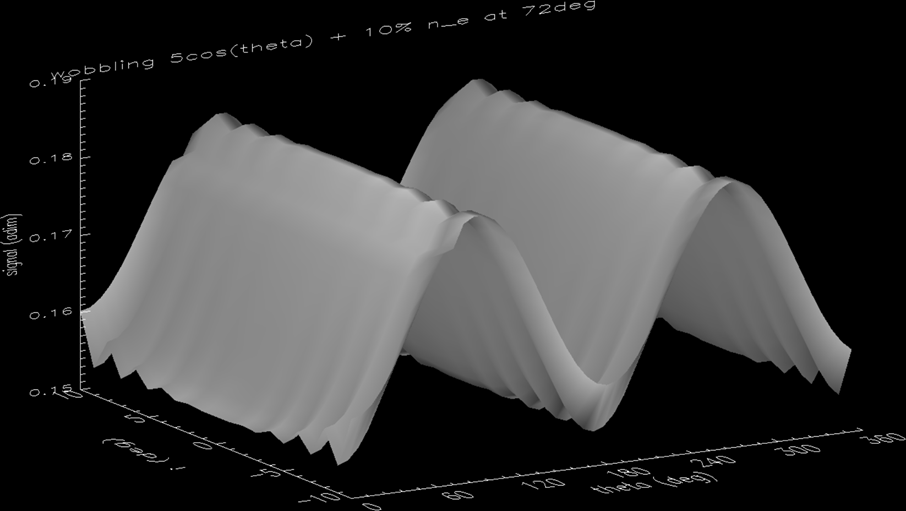
\includegraphics[width=0.6\linewidth]{hwp_wobbling.png}
\caption{2$f$ signal from a (1,0,0,0) Stokes vector incident on a Sapphire HWP wobbling with the incoming radiation varying with the law $5\cos(i)$ with $i$ the incident angle of the incoming radiation.}
\label{hwpwobble}
\end{figure}

\paragraph{Parameterization:}
The most naive way to parameterize the HWP wobbling is assuming an incident angle varying with a co-sinusoidal law. Since the normal to the HWP and the disc are perpendicular each other, the variation with time of the HWP disc can be translated
into variation of the incident angle. Since it is highly unlikely that a wobbling effect will keep the same amplitude across time, a more realistic parameterization of this effect should consider injecting random angle fluctuations as well. \textbf{These can be translated into 2$f$ and 4$f$ signals through.... to determine the scientific impact of the wobble and to develop quality control specifications.}
